\chapter{Clystyru $k$-cymedrau}\label{cha:literature}
\section{Cefndir}\label{sec:axelrodoriginal}
Mae clystyru $k$-cymedrau yn ffordd o ddysgu heb oruchwyliaeth, mae'n cymeryd data heb ei labelu ac yn eu sortio i fewn i $k$ wahanol clystyrau yn yr obaith i darganfod rhyw strwythyr doedden ddim yn gwybod gynharach.

\begin{figure}
\begin{center}
\begin{minipage}{.4\linewidth}
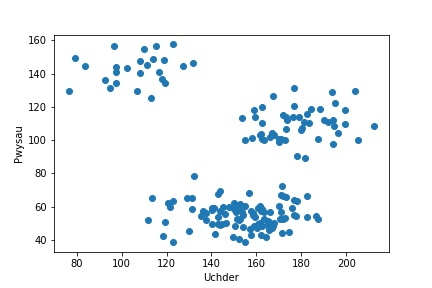
\includegraphics[width=1\linewidth]{../img/Scatterpython.jpeg}
\end{minipage}%
\begin{minipage}{1cm}
$\Rightarrow$
\end{minipage}%
\begin{minipage}{.4\linewidth}
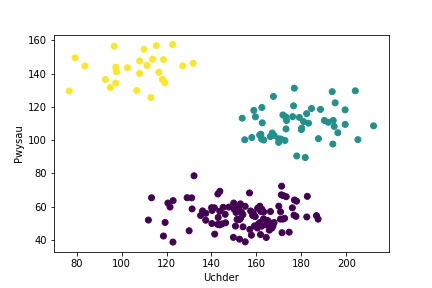
\includegraphics[width=1\linewidth]{../img/3clystwrpython.jpeg}
\end{minipage}%
\label{fig:Cefndir_Clysteru_k_modd}
\caption{Cyn ac ar \^{o}l clystyru $k$-cymedr.}
\end{center}
\end{figure}

I rhoi enghraifft i'r llun uchod, mae'r gwerthoedd ar echelin $x$ yn cynrychioli uchder rhyw person ag yr llall yn cynrychioli pwysau y person. Fel welwn yn Darlun~\ref{fig:Cefndir_Clysteru_k_modd} gallwn weld tri grwp naturiol wedi'i ffurfio. Rydym nawr eisiau eu grwpio yn ffurf Mathemategol. Fysa clystyru $k$-cymedrau medru dosrannu y tri grwp fel welwn ar ochr dde y darlun. 

%%Adio mwy ar sut a pam mae'n cael ei ddefnyddio..

\section{Sut mae Clystyru $K$-cymedrau yn gweithio?}

\subsection{Y Dull}

Mae clystyru $k$-cymedrau yn syml, mae dim ond yn dilyn pedwar cam(REFERENCE)! I wneud yn siwr fod yn ei ffyrf fwyaf cyntefig, fyddan yn defnyddio mesur pellter Ewclidaidd. Yn ogystal fydd rhaid dewis $k$ cyn cychwyn y proses. Mae'n bosib optimeiddio y dewis o $k$, wnawn trafod am hyn hwyrach ymlaen. Dyma pedwar cam yr algorithm a sut fyddym yn edrych pan fyddwn ni yn ei ymgeisio'r algorithm ar y data welwn yn \ref{fig:Cefndir_Clysteru_k_modd}:

\begin{enumerate}
\item Aseinio pob elfen i un o'r $k$ clystyrau ar hap.

\begin{figure}[h]
\begin{center}
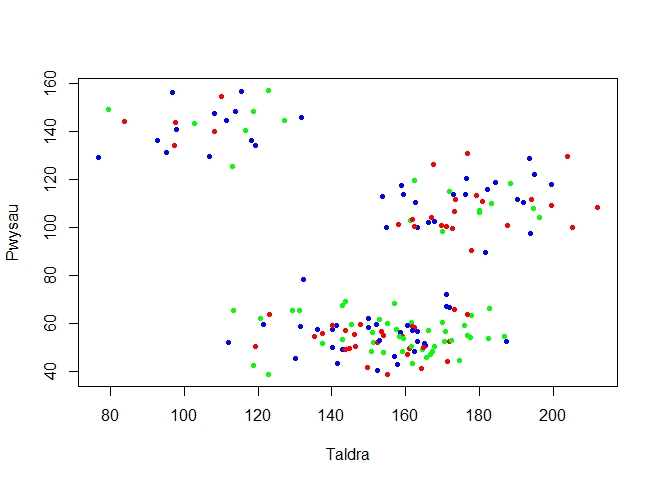
\includegraphics[width=0.5\linewidth]{../img/Cam1.jpeg}
\end{center}
\end{figure}

\item Cyfrifo y cymedr pob clwstwr.

\begin{figure}[h]
\begin{center}
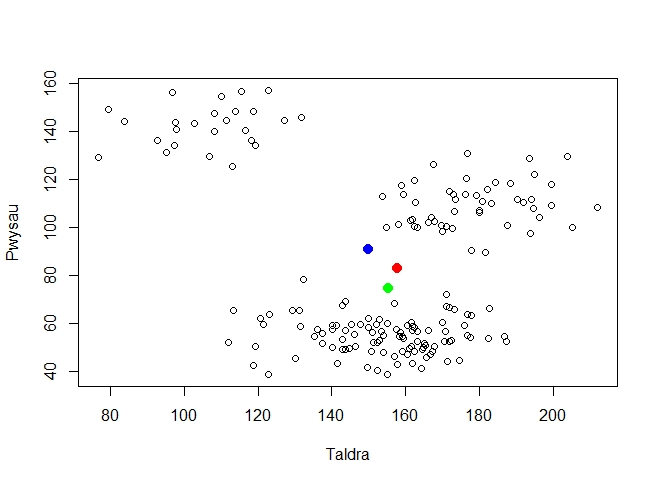
\includegraphics[width=0.5\linewidth]{../img/ClystyrauCychwynol.jpeg}
\end{center}
\end{figure}

\item Aseinio pob elfen unwaith eto i'r clwstwr gydag cymedr agosaf.

\begin{figure}[h]
\begin{center}
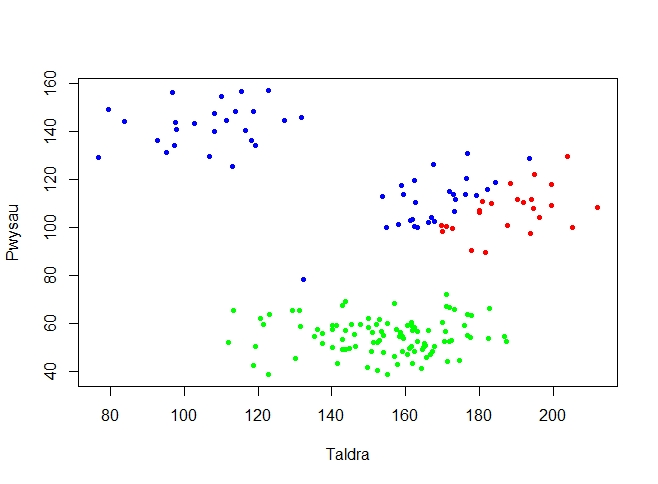
\includegraphics[width=0.5\linewidth]{../img/Cam3.jpeg}
\end{center}
\end{figure}

\item Ailadrodd camau dau a tri tan fod y creiddiau ddim yn symyd unrhyw mwy.

\begin{figure}[h]
\begin{center}
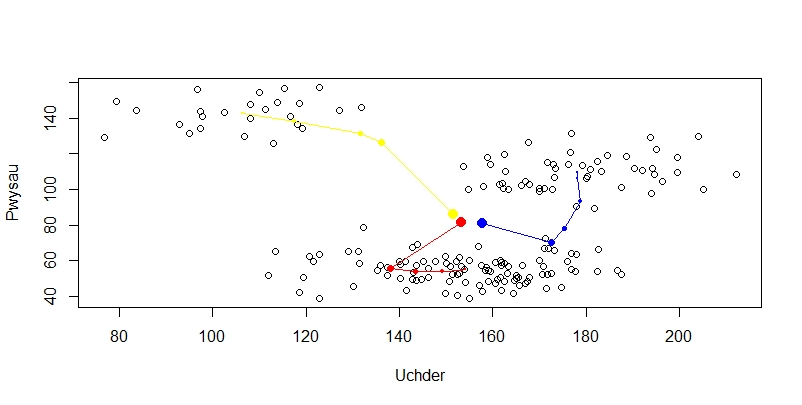
\includegraphics[width=0.5\linewidth]{../img/Convergence4.jpeg}
\end{center}
\end{figure}

\end{enumerate}  

\subsection{Darn Mathemategol}

Diffiniwn pob clwstwr rydym yn ceisio darganfod fel $C_i$ lle bydd i $\in \{ 1, 2, \dots, k\}$, mae gennym hefyd $n$ pwyntiau data $x_1,x_2,\dots,x_n$. Y darn gyntaf fydd i aseinio phob $x_j$ i rhyw clwstwr $C_i$ ar hap. Yna gan ein fod yn datgelu ein fod yn delio gydag pl\^{a}n Ewclidaidd, mi fyddym yn delio gyda darganfod cymedr pob clwstwr gan y fformiwla canlynol:
Diffiniwn $S_i$ fel y set o pwyntiau data sydd wedi'i aseinio i clwstwr $C_i$.
$$ C_i = \frac{1}{|S_i|}\sum_{x_j \in S_i} {x_j} $$
Nawr mae pob clwstwr gyda cymedr newydd, fedrym aseinio pob pwynt data i'r craidd agosaf. Fydd hyn yn cael ei gwneud gan mynd drwy pob pwynt data ag cyfrifo y pellter Ewlcidaidd i phob craidd. Yna fydd y pwynt priodol yn cael ei labelu gyda y clwstwr gyda pellter lleiaf o'r craidd ir pwynt data.
$$ \arg \min_{c_i} dist(c_i,x_j)^2$$
Unwaith mae'r proses wedi'i cychwyn, does dim ond angen ailadrodd y darn o darganfod y creiddiau newydd ag yna ail labelu'r pwyntiau data.


\subsection{Sut i ddarganfod y $K$ orau?}

Mae yna wahanol ffurf i ddarganfod $K$, wnawn edrych ar ddau wahanol ffordd o gwneud hyn. 

\subsubsection{Dull Penelin}

Mae'r dull penelin yn cymharu'r cyfanswm o swm sgwariau o fewn y clystyrau. Unwaith gennym yr cyfanswm o swm sgwariau o fewn clystyrau i phob $k$ rydym eisiau cymharu; fyddem yn creu plot o phob $k$ yn erbyn eu cyfanswm o swm sgwariau o fewn y clystyrau. Unwaith mae gennym y graff, allwn ei ddadansoddi. 

\begin{figure}[h]
\begin{center}
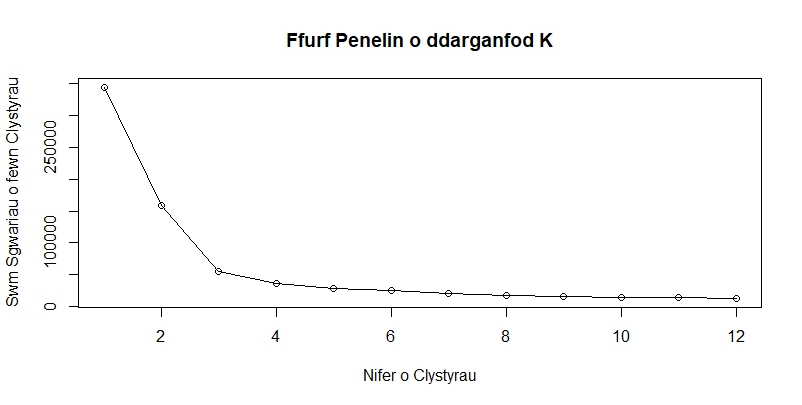
\includegraphics[width=0.5\linewidth]{../img/Dull_Penelin.jpeg}
\end{center}
\end{figure}

Yn y graff uchod sydd gennym, fydd yn dangos sut mae'r swm sgwariau yn mawr yn cychwyn gyda $k$ sydd yn gwneud synnwyr. O'r pwynt yma wedyn fydd yna newid ystyrlon yn y swm sgwariau. Unwaith mae'r newid ystyrlon yn dod i ben fydd gennym ongl yn cael ei greu lle bydd newid $K$ dim ond yn creu newid ymylol. Y pwynt yma fydd yr optimwm nifer o $K$. Fel gwelwn yn glir yn ein enghraifft ni, mae'n glir fod $K$=3 yw dewis orau ar $K$.

\subsubsection{Dendrogram}

\begin{figure}[h]
\begin{center}
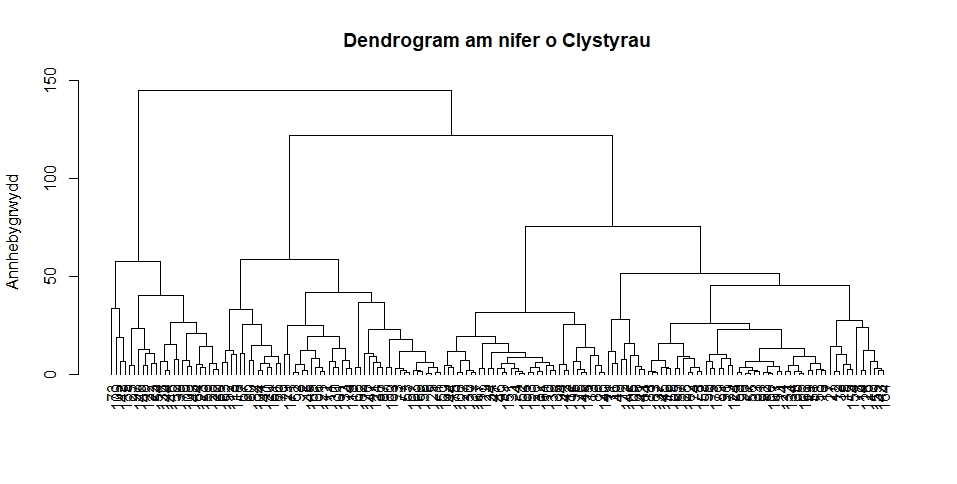
\includegraphics[width=0.5\linewidth]{../img/Dendrogram.jpeg}
\end{center}
\end{figure}

\section{Tiwtorial yn R}
Mi fyddwn yn edrych ar ddata o uchder a pwysau 175 wahanol person. Mi allwch chi lawrlwytho y data yma o fan hyn (INSERT LINK HERE). 

Yno fydd angen lawrlwytho a gosod y pecynnau "graphics", "stats" ag "datasets" ar eich fersiwn chi o R studio. Ffordd hawdd i gwirio hyn fydd i ddefnyddio y c\^{o}d canlynol:

\begin{minted}{r}
install.packages("graphics")
install.packages("stats")
install.packages("datasets")
library(graphics)
library(stats)
library(datasets)
\end{minted}
Mae'r darn gynta o'r c\^{o}d uchod yn gosod/diweddaru y pecynnau angenrheidiol. Mae'r ail darn yn llwytho'r pecynnau i ein fersiwn ni o R Studio.

Nawr mi wnawn mewnforio y data. 

\begin{minted}{r}
heightvsweight <- read.csv("C:/Users/User/Desktop/Dysgu_Peirianyddol/heightvsweight.csv")
View(heightvsweight)
\end{minted}

Fydd rhaid wneud yn siwr fod eich cyfeiriadur yn gywir i'r lleoliad o eich ffeil chi.
Ar ol rhedeg y c\^{o}d ddylsai tabl agor mewn arwahan. Ddylsai edrych yn debyg i'r canlynol:

\begin{figure}[h!]
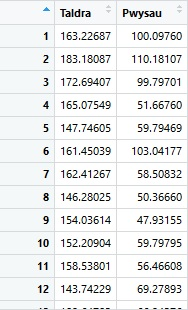
\includegraphics[width=0.35\linewidth]{../img/Data_yn_R.jpg}
\label{fig:DataR}
\end{figure}

Gan fod y data hefo enwau ar gyfer y colofnau, gallwn atodi y data i llwybr chwilio R. Bydd hyn yn gadael i ni cyfeirio i enwau colofnau y data yn ein c\^{o}d fydd yn gwneud yn lawer mwy symlach i ddeallt.

\begin{minted}{r}
attach(heightvsweight)
\end{minted}

I gwneud fwy o synwyr o'r data, mi wnawn plotio'r data. Wnawn weld fod yna 3 clwstwr glir. 

\begin{minted}{r}
plot(Uchder, Pwysau, pch = 21)
\end{minted}

\begin{figure}[h]
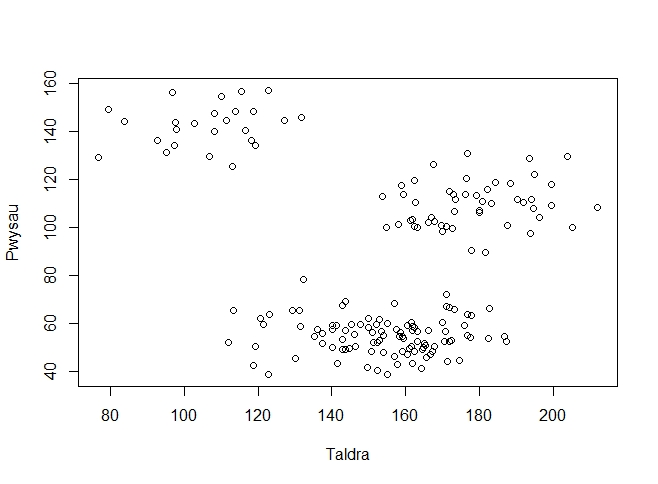
\includegraphics[width=0.5\linewidth]{../img/ScatterplotR.jpeg}
\label{fig:ScatterplotR}
\end{figure}

Rwan rydym yn gallu gweld fod y data yn gallu cael i rhannu i dair clwstwr wahanol, mi wnawn defnyddio y ffyrf mathemategol i'w ddehongli. Rhedwn y canlynol i rhedeg clystyru $k$-cymedrau yn R. Rydym yn defnyddio yr ymresymiad "nstart" i ddewis faint o setiau ar hap o creiddiau wnawn gymeryd. (REFERENCE O SUT MAE FFORMIWLA YN GWEITHIO) 

\begin{minted}{r}
kcymedr <- kmeans(heightvsweight,3, nstart = 50)
\end{minted}

Allwn nawr adio colofn newydd ir data sef y clystyrau newydd mae'r algorithm wedi'i darganfod.

\begin{minted}{r}
heightvsweight$Clwstwr3 <- kcymedr$cluster
\end{minted}

Gallwn weld yr newid hyn gan defnyddio'r c\^{o}d o gynnar.

\begin{minted}{r}
View(heightvsweight)
\end{minted}

\begin{figure}[h]
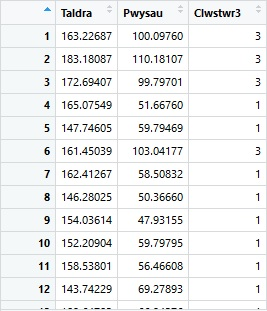
\includegraphics[width=0.5\linewidth]{../img/Data3_yn_R.jpg}
\end{figure}

Mae'n bosib fydd yr algorithm wedi rhoi rhif wahanol ar gyfer clystyrau wahanol ond ddylsai yr clystyrau fod yn hafal. Mae hyn oherwydd y setiau ar hap mae'r fformiwla yn ei gymeryd yn cychwyn.

Rhedwn y c\^{o}d canlynol i cael gweld y clystyrau newydd ar graff.

\begin{minted}{r}
plot(Uchder, Pwysau, pch = 21, bg=c("red","green","blue")[unclass(kcymedr$cluster)])
\end{minted}

\begin{figure}[h]
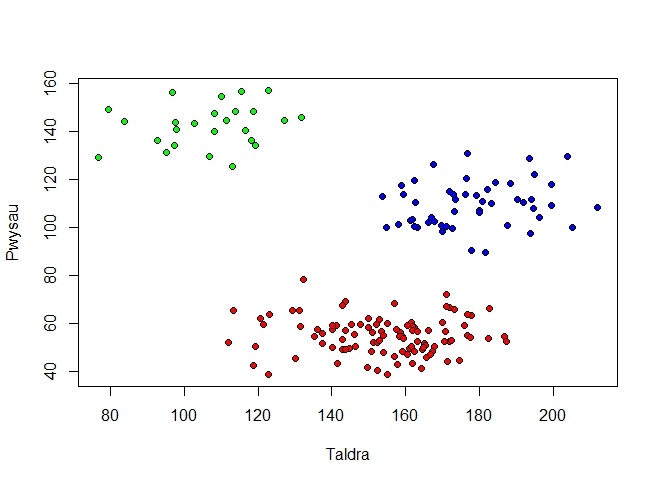
\includegraphics[width=0.5\linewidth]{../img/3clwstwrR.jpeg}
\end{figure}

Y nawr mi nawn rhedeg yr algorithm ar gyfer 6 clwstwr i weld yr clystyrau pan fydd $k$=6. 

\begin{minted}{r}
kcymedr <- kmeans(heightvsweight,6, nstart = 50)
heightvsweight$Clwstwr6 <- kcymedr$cluster
View(heightvsweight)
\end{minted}

\begin{figure}[h]
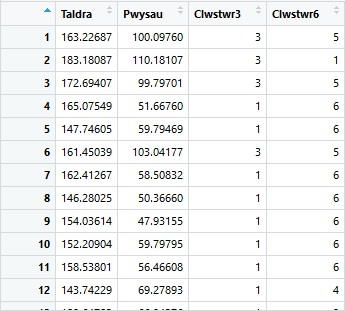
\includegraphics[width=0.5\linewidth]{../img/Data6_yn_R.jpg}
\end{figure}

Gwelwn fod yr labelau newydd wedi cael ei ychwanegu i ein tabl. Yna gan plotio graff arall, fedrym weld y 6 clwstwr yn gliriach.

\begin{minted}{r}
plot(Uchder, Pwysau, pch = 21, bg=c("red","green","blue", "yellow", "black", "white")[unclass(kcymedr$cluster)])
\end{minted}

\begin{figure}[h]
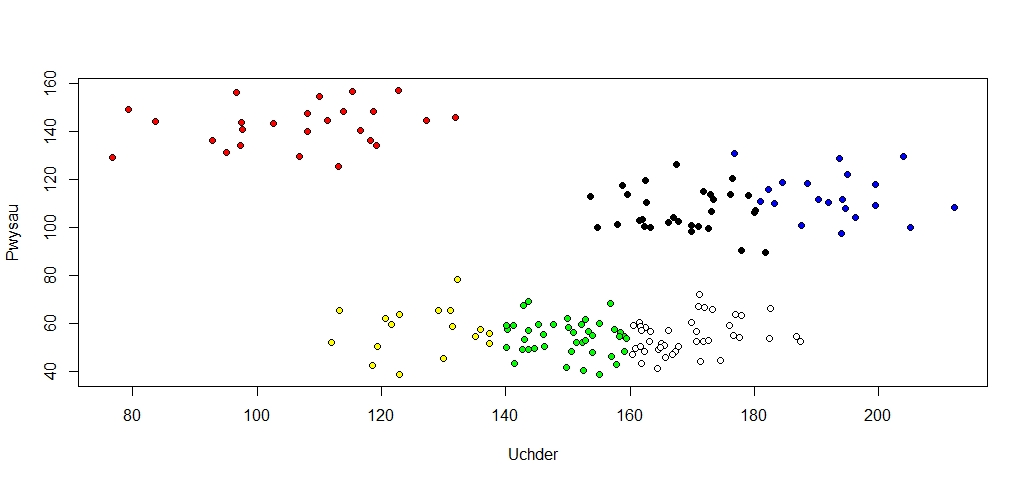
\includegraphics[width=0.5\linewidth]{../img/6clwstwrR.jpeg}
\end{figure}


%Mae'r data iris ar gael iddym drwy'r pecyn "datasets". Yn yr enghraifft top mi wnaethom defnyddio k fel 3, felly hyna be wnawn neud eto.
%Dyma'r c\^{o}d ar gyfer rhedeg clystyru k-cymedrau:
%\begin{minted}{r}
%clysteru_tri <- kmeans(iris[,1:4],3, nstart = 20)
%clysteru_tri 
%\end{minted}
%Mae'r llinell gyntaf o c\^{o}d yn rhedeg clystyru k-cymedrau ar y set data iris gyda k=3. Mae'r darn nstart yn cynrychioli faint o dosraniadau i drio yn cychwyn yn erbyn'r ffwythiant amcan, er mwyn dewis y cychwyn orau. Mae'r ail linell yn allbwn yr wybodaeth canlynol:
%\begin{minted}{r}
%>>>K-means clustering with 3 clusters of sizes 50, 62, 38
%>>>
%>>>Cluster means:
%>>>  Sepal.Length Sepal.Width Petal.Length
%>>>1     5.006000    3.428000     1.462000
%>>>2     5.901613    2.748387     4.393548
%>>>3     6.850000    3.073684     5.742105
%>>>  Petal.Width
%>>>1    0.246000
%>>>2    1.433871
%>>>3    2.071053
%>>>
%>>>Clustering vector:
%>>>  [1] 1 1 1 1 1 1 1 1 1 1 1 1 1 1 1 1 1 1 1 1 1 1
%>>> [23] 1 1 1 1 1 1 1 1 1 1 1 1 1 1 1 1 1 1 1 1 1 1
%>>> [45] 1 1 1 1 1 1 2 2 3 2 2 2 2 2 2 2 2 2 2 2 2 2
%>>> [67] 2 2 2 2 2 2 2 2 2 2 2 3 2 2 2 2 2 2 2 2 2 2
%>>> [89] 2 2 2 2 2 2 2 2 2 2 2 2 3 2 3 3 3 3 2 3 3 3
%>>>[111] 3 3 3 2 2 3 3 3 3 2 3 2 3 2 3 3 2 2 3 3 3 3
%>>>[133] 3 2 3 3 3 3 2 3 3 3 2 3 3 3 2 3 3 2
%>>>
%>>>Within cluster sum of squares by cluster:
%>>>[1] 15.15100 39.82097 23.87947
%>>> (between_SS / total_SS =  88.4 %)
%\end{minted}
%Mae'r c\^{o}d uchod rhoi pob wybodaeth a fysa chi eisiau wybod fel allbwn o'r proses.
%I weld y clysterau allwn plotio graff ar gyfer phob cyfuniad o newidynnau. Mae hyn yn alluogi ni i weld yr gwaith dpsbarthu mae'r algorithm wedi'i neud.
%\begin{minted}{r}
%plot(iris[,1:4], pch = 24, bg=c("red","green3","blue")[unclass(clysteru_tri$cluster)])
%\end{minted}
%Yn y ffwythiant "plot" uchod, mae'r darn gynta ohono yn cyfeirio tuag at pa data fydd yn cael ei clysteru. Mae'r ail darn yn penodi be fydd pob pwynt data yn cael ei cynrychioli fel pan %mae'r darn dwythaf yn penodi lliw i pob clwstwr.

%Mi wnawn edrych y nawr ar yr set data iris sy'n boblogaidd iawn yn y maes ystadegaeth a gwyddor data. Mae'r data yn cynnwys mesuriadau uchder ag lled petal a setal 150 planhigyn iris. Yn isod gweler lun o allbwn clystyru k-cymedrau yn erbyn y clystyrau gwreiddiol o'r data. Gwelwyd fod yr algorithm yn neud yn wych!


\section{Tiwtorial yn python}
Yn y tiwtorial hyn mi wnawn edrych ar yr un data a welom yn y tiwtorial dwythaf.
I gychwyn fydd rhaid mewnforio y pecynnau pandas, matplotlib.pyplot ag sklearn.cluster drwy rhedeg y c\^{o}d canlynol:

\begin{minted}{python}
import pandas as pd
import matplotlib.pyplot as plt
import sklearn.cluster
\end{minted}

Yr rwan mi wnawn mewnforio y data (INSERT LINK HERE) i fewn i ein gwaith gan rhedeg y c\^{o}d:
\begin{minted}{python}
data = pd.read_csv('heightvsweight.csv')
\end{minted}
Fydd rhaid gwneud yn siwr fod y data wedi cael ei gadw yn yr un cyfeiriadur ag yr ffeil rydych yn ei ddefnyddio i rhedeg y c\^{o}d.
Unwaith fydd wedi cael ei mewnforio, all ni gweld yn fras y ddata gennym ni. 
\begin{minted}{python}
data.head()
\end{minted}

\begin{figure}
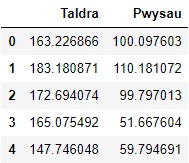
\includegraphics[width=0.35\linewidth]{../img/tabl1.jpg}
\label{fig:Data1}
\end{figure}

I weld y ddata mewn ffordd fwy gweledol, wnawn plotio graff gwasgariad o'r data

\begin{minted}{python}
plt.scatter(data['Uchder'], data['Pwysau']);
plt.xlabel('Uchder')
plt.ylabel('Pwysau')
plt.show()
\end{minted}

\begin{figure}[h!]
\begin{center}
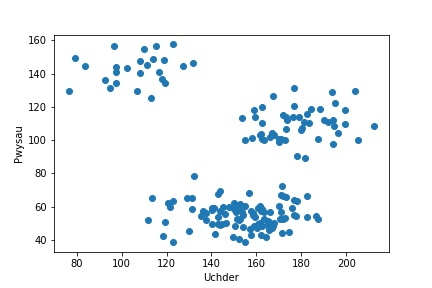
\includegraphics[width=0.7\linewidth]{../img/Scatterpython.jpeg}
\caption{Enghraifft o ddata da i cael ei clystyru.}
\label{fig:Scatterpython}
\end{center}
\end{figure}

Fel gwelwn, mae'r data yn edrych fel ei fod mewn tri clystwr. Felly wnawn defnyddio y ffyrf mathemategol i ddarparu arnyn nhw.

\begin{minted}{python}
kmeans = sklearn.cluster.KMeans(n_clusters=3).fit(data)
data['Cluster (k=3)'] = kmeans.predict(data)
\end{minted}



\begin{minted}{python}
data.head()
\end{minted}

\begin{figure}[h!]
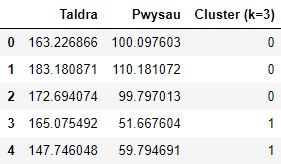
\includegraphics[width=0.35\linewidth]{../img/tabl2.jpg}
\label{fig:Data2}
\end{figure}

Fel y gwelwyd, mae'r data wedi'i rhoi i fewn clwstwr a wedi'i labelu gyda rhif y clystwr. Gan bod pob pwynt yn y data nawr gyda label, allwn ni creu y plot eto ond gyda bob clystwr yn lliw gwahanol.

\begin{minted}{python}
plt.scatter(data['Uchder'], data['Pwysau'], c=data['Cluster (k=3)']);
plt.xlabel('Uchder')
plt.ylabel('Pwysau')
plt.show()
\end{minted}

\begin{figure}[h!]
\begin{center}
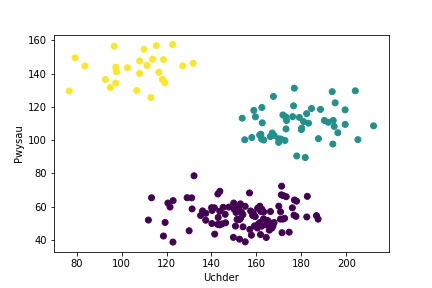
\includegraphics[width=0.7\linewidth]{../img/3clystwrpython.jpeg}
\caption{Sut ddylsa eich graff edrych gyda 3 clystwr.}
\label{fig:3clystwrpython}
\end{center}
\end{figure}

Fel y gwelwn, gweithiodd yr algorithm yn wych, wnawn nawr trio clysteru $k$-cymedrau gyda $k$ yn hafal i 6.

\begin{minted}{python}
kmeans = sklearn.cluster.KMeans(n_clusters=6).fit(data)
data['Cluster (k=6)'] = kmeans.predict(data)
\end{minted}

\begin{minted}{python}
data.head()
\end{minted}

\begin{figure}[h!]
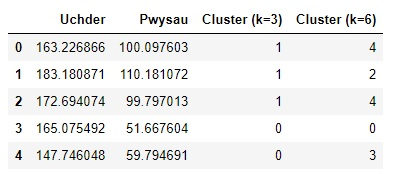
\includegraphics[width=0.35\linewidth]{../img/tabl3.jpg}
\label{fig:Data3}
\end{figure}

Gwelwn caiff y ddata yn ogystal ei rhoi i fewn i 6 clwystwr wahanol. 

\begin{minted}{python}
plt.scatter(data['Uchder'], data['Pwysau'], c=data['Cluster (k=6)']);
plt.xlabel('Uchder')
plt.ylabel('Pwysau')
plt.show()
\end{minted}

\begin{figure}[h!]
\begin{center}
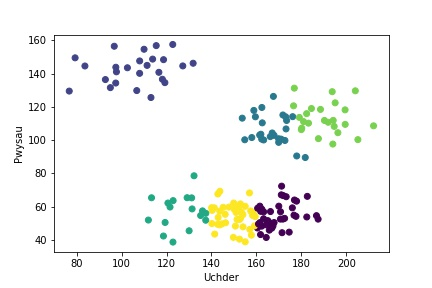
\includegraphics[width=0.7\linewidth]{../img/6clystwrpython.jpeg}
\caption{Sut ddylsa eich graff edrych gyda 6 clystwr.}
\label{fig:6clystwrpython}
\end{center}
\end{figure}

Dyma sut dylsa eich ddata edrych fel ar ol a prosesu drwy clysteru 6-cymedrau. 
